\documentclass[a4paper, twocolumn, html, DIV=12]{scrartcl}

\usepackage[T1]{fontenc}
\usepackage[utf8]{inputenc}
\usepackage[british]{babel}

\addtokomafont{disposition}{\rmfamily}
\addtokomafont{descriptionlabel}{\rmfamily}

\usepackage{amsmath}
\usepackage{amssymb}

\usepackage{todonotes}

\usepackage{booktabs}
\usepackage{hyperref}

\usepackage{graphicx}
\usepackage{subcaption}

%\usepackage[pdftitle={Implementation of iPMCMC in Monad-Bayes},
  %pdfauthor={Per Engström},
  %pdffitwindow=true,
  %breaklinks=true,
  %colorlinks=true,
  %urlcolor=blue,
  %linkcolor=red,
  %citecolor=red,
  %anchorcolor=red]{hyperref}
%\usepackage{pdfpages}
%\usepackage{algorithm}
%\usepackage{algorithmic}
%\usepackage{natbib}


\usepackage{minted}
\usemintedstyle{solarizedlight}
\usepackage{mdframed}
\surroundwithmdframed{minted}

\setminted[Haskell]{fontsize=\footnotesize}


\usepackage{tikz}
\usetikzlibrary{positioning,backgrounds,matrix}
\definecolor{sbase3}{HTML}{FDF6E3}

\usepackage[font={small,sf}]{caption}

\usepackage[sorting=nty,style=numeric]{biblatex}
\bibliography{references}



\title{Interacting Particle Inference for Probabilistic Programing in Haskell}

\author{Per Engström}

\date{\today}

\begin{document}
\twocolumn[
  \begin{@twocolumnfalse}
    \maketitle
    \begin{abstract}
Probabilistic programming shows much promise as a declarative way to define statistical models, but inference is often expensive. A parallelisable particle MMCMC sampler is implemeted in Haskell and the DSL Monad-Bayes. The method shows good performace compared to a single SMC sampler, but the full potential of the method could not be manifested.
    \end{abstract}
  \end{@twocolumnfalse}
]


\section{Introduction}

Bayes' theorem
\begin{equation}
    \Pr(\theta\mid D) = \frac {\Pr(\theta) \Pr(D \mid \theta)}{\Pr(D)}
\end{equation}
about conditional probability is well-known from any introductory course on probability theory. It expresses how one's prior believed distribution of $\theta$ ($\Pr(\theta)$) is updated given observations $D$ into a posterior belief $\Pr(\theta\mid D)$. The likelihood $\Pr(D \mid \theta)$ represents the probability of generating the observation $D$ given a particular $\theta$. The marginal likelihood $\Pr(D)$ acts as normalisation to ensure the distribution is valid.

The posterior distribution is valuable as it enables prediction from observations. However, unless the prior and likelihood are simple distributions then the posterior is often intractable~\cite{barber} requiring numerical methods to sample from. One approach for approximating complicated posteriors is the family of MCMC  methods~\cite{robert}. The particle Markov chain Monte Carlo methods by Andrieu et al.~\cite{pmcmc}, and in particular the particle Gibbs (PG) sampler, aims to improve the proposals for the MCMC sampler by using importance sampling in the form of sequential Monte Carlo (SMC)~\cite{smc}. The PG sampler uses a modified SMC sampler conditioned on an existing particle trajectory, conditional SMC (CSMC).

The CSMC sampler is prone to path degeneracy. If the resampling collapses then, by design, only the conditional trajectory remains, reducing the mixing required for a healthy MCMC step. Rainforth et al.~\cite{ipmcmc} proposes a solution calle Interacting Particle Markov Chain Monte Carlo (iPMCMC) where several CSMC and SMC sampler are run in parallel. By sampling the conditional trajectories possibly from independent (unconditional) SMC samplers the mixing is improved. In addition, the nodes only interact briefly promising a high degree of parallelisation.

This thesis presents a Haskell implementation of the iPMCMC sampler for Bayesian inference in the probabilistic programming DSL Monad-Bayes~\cite{mbayes}. Haskell\footnote{\url{https://www.haskell.org}} is a general-purpose purely functional lazy programming language. To readers unfamiliar with the language an introductory text is recommended~\cite{haskell}. The monad abstraction for structured computation is well-suited for DSLs, and type classes allows flexible implementation of probabilistic functionality and inference.

\subsection{Probabilistic programming}
\label{sec:pprog}

One promising way to express statistical models, and in particular Bayesian problems is probabilistic programming~\cite{dippl}. This paradigm leverages the expressiveness and familiarity of programming
languages  to define models independently of inference, allowing the models to be composable.

In the design of a probabilistic language the main trade-off is between
expressiveness and performance of inference. A restricted language like
BUGS~\cite{bugs} makes the inference simpler. In universal
(Turing-complete) languages like Anglican~\cite{anglican} and
Monad-Bayes~\cite{mbayes} the inference is more challenging.

Central to all probabilistic languages is the ability to construct more
complex models using simpler building blocks, usually primitive distributions
and use Bayesian filtering. Consider the problem of regression of some complicated function $y = f(\theta,x)$ parametrised by a parameter $\theta > 0$ and observations $D = \{ (x_i,y_i) \}_{i=1}^N$ influenced by some normal noise $\delta \sim \operatorname{Norm}(0,1)$ such that
\begin{equation}
   y_i = f(\theta;x_i) + \delta .
\end{equation}
In Bayesian modelling, we want to find the distribution for the parameter $\theta$ given the data $D$, i.e. $\Pr(\theta \mid D)$. If the function is implemented as
\begin{minted}{Haskell}
f :: Double -- theta
  -> Double -- x
  -> Double -- y
\end{minted}
then assuming a prior $\Pr(\theta) \sim \operatorname{Gamma}(1,1)$, the model is also a function taking the list of observations
\begin{minted}[linenos]{Haskell}
reg :: MonadInfer m
  => [(Double,Double)] -- Observations
  -> m Double
reg obs = do
  theta <- gamma 1 1
  let fun = f theta
      sigma = 1
  forM obs (\ (x,y) -> do
    let mu = fun x
        p = normalPdf mu sigma y
    score p)
  return theta
\end{minted}
where we for each observation score the likelihood---how probable the data is given the parameter (line 10)---skewing the prior distribution (line 7) favouring values close to where the error is small. Note how the formulation closely matches the mathematical definition. This thesis will focus on efficient but approximate sampling-based
methods for finding the distribution in such problems by implementing the iPMCMC sampler and evaluating the parallelisation and comparing it to samplers in Monad-Bayes.



\section{Theory}

This section contains the necessary theory behind inference and probabilistic programs as well as details how the Monad-Bayes library works and a description of the iPMCMC method.

\subsection{Inference on probabilistic programs}
\label{sub:inference_on_probabilistic_programs}

\begin{figure}[h!]
\begin{center}
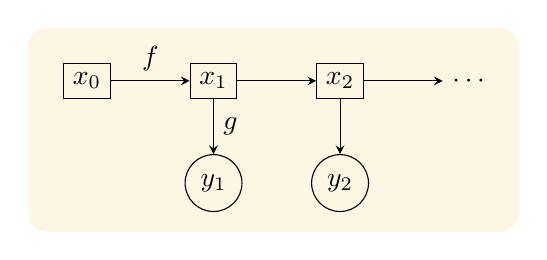
\begin{tikzpicture}[scale=1, transform shape]
    \node[draw] (x0) {$x_0$};
    \node[draw, right=of x0] (x1) {$x_1$};
    \node[draw, right=of x1] (x2) {$x_2$};
    \node[right=of x2] (x3) {$\cdots$};

    \node[draw, circle, below=2em of x1] (y1) {$y_1$};
    \node[draw, circle, below=2em of x2] (y2) {$y_2$};

    \path[-stealth]
    (x0) edge node[above] {$f$} (x1)
    (x1) edge  (x2)
    (x2) edge  (x3)
    (x1) edge node[right] {$g$} (y1)
    (x2) edge  (y2);

    \begin{pgfonlayer}{background}
        \filldraw [line width=5mm,join=round,sbase3] (x0.north west) ++ (-2mm,2mm) rectangle
        (y2.south -| x3.east);
    \end{pgfonlayer}
\end{tikzpicture}
\end{center}
\caption{A diagram of a hidden markov process.}
\label{fig:hmm}
\end{figure}

A hidden Markov model is a construct of some hidden state $x_t$ evolving by some known process $f(x_t \mid x_{t-1})$ and $\mu(x_0)$ where both functions should be seen as distributions. In other words, the value of $x_t$ is not known, but the underlying process is. In addition, some observations $y_t$ \emph{are} known together with their emission process $g(y_t \mid x_t)$, see figure~\ref{fig:hmm}. By comparing the measured values $y_t$ with their distribution $g$ and proposed hidden values $x_t$ it is possible to score the proposals and use the scores $w_t$ to find the most likely values.

\begin{figure}[h!]
\begin{center}
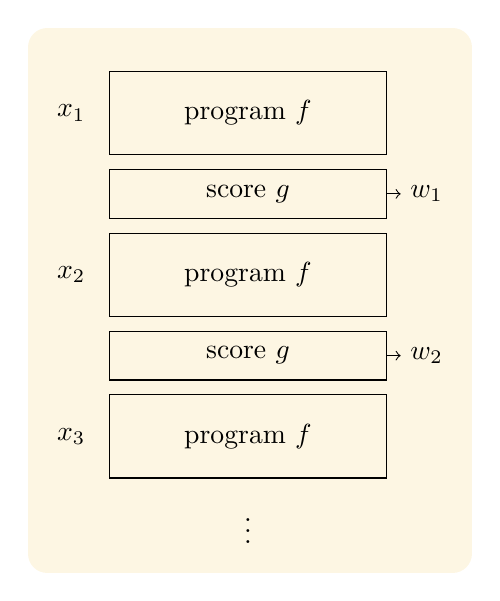
\begin{tikzpicture}[scale=1, transform shape,node distance=0.5em]
    \node[minimum width=10em,minimum height=3em,draw] (x1) {program $f$};
    \node[minimum width=10em,draw,below=of x1,inner sep=2mm] (y1) {score $g$};
    \node[minimum width=10em,minimum height=3em,draw,below=of y1] (x2) {program $f$};
    \node[minimum width=10em,draw,below=of x2,inner sep=2mm] (y2) {score $g$};
    \node[minimum width=10em,minimum height=3em,draw,below=of y2] (x3) {program $f$};

    \node[left=of x1] {$x_1$};
    \node[left=of x2] {$x_2$};
    \node[left=of x3] (xx3) {$x_3$};

    \node[right= of y1] (w1) {$w_1$};
    \node[right= of y2] (w2) {$w_2$};

    \node[below=of x3] (dots) {$\vdots$};

    \path[->]
    (y1) edge (w1)
    (y2) edge (w2);

    \begin{pgfonlayer}{background}
        \filldraw [line width=5mm,join=round,sbase3] (x1.north -| w1.east) ++ (0,3mm) rectangle
        (dots.south -| xx3.west);
    \end{pgfonlayer}
\end{tikzpicture}
\end{center}
\caption{A program seen as a hidden Markov model.}
\label{fig:hmmprog}
\end{figure}


In the context of models expressed as probabilistic programs the time aspect is more accurately viewed as the execution of the program as seen in figure~\ref{fig:hmmprog}. As the program executes random variables are sampled and manipulated. This corresponds to $f$ above. The program is interrupted at various points by scoring the current execution path, possibly depending on the sampled values. This is the likelihood score and the method for determining the score is model-dependent on $g$. These scorings separates the programs into parts, the $x_t$'s.

\subsubsection{SMC and CSMC}
\label{ssub:smc_and_csmc}



\begin{figure}[h]
\begin{center}
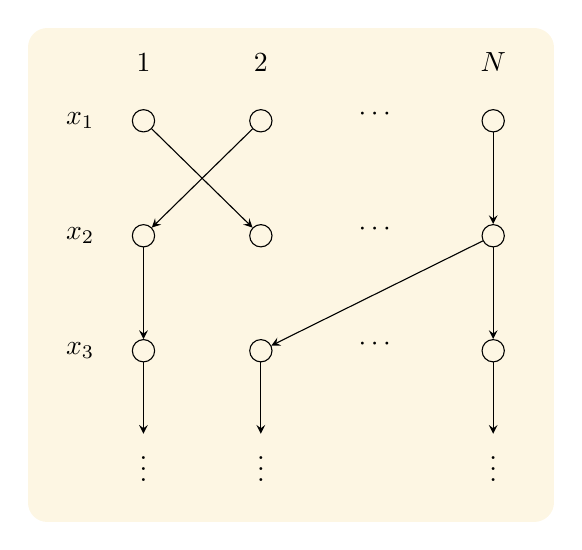
\begin{tikzpicture}[node distance=1em,scale=1, transform shape,smcnode/.style={circle,draw,inner sep=1mm}]
    \matrix (m) [matrix of nodes,nodes in empty cells, nodes={smcnode}, row sep=2em, column sep=2em]
    {  &  & \node[draw=none] {$\cdots$};  &  \\
       &  & \node[draw=none] {$\cdots$};  &  \\
       &  & \node[draw=none] {$\cdots$};  &  \\
      \node[draw=none] {$\vdots$}; &\node [draw=none]{$\vdots$}; & \node[draw=none] {}; & \node [draw=none]{$\vdots$}; \\
      };

      \path[-stealth]
      (m-3-4) edge ++(0,-3em)
      (m-3-2) edge ++(0,-3em)
      (m-3-1) edge ++(0,-3em)
      (m-2-4) edge (m-3-4)
      (m-2-4) edge (m-3-2)
      (m-2-1) edge (m-3-1)
      (m-1-4) edge (m-2-4)
      (m-1-1) edge (m-2-2)
      (m-1-2) edge (m-2-1);

      \node[left=of m-1-1] {$x_1$};
      \node[left=of m-2-1] {$x_2$};
      \node[left=of m-3-1] {$x_3$};

      \node[above=of m-1-1] {$1$};
      \node[above=of m-1-2] {$2$};
      \node[above=of m-1-4] {$N$};

    \begin{pgfonlayer}{background}
        \filldraw [line width=5mm,join=round,sbase3] (m.north west) ++ (-2em,1em) rectangle
        (m.south east);
    \end{pgfonlayer}
\end{tikzpicture}
\end{center}
\caption{Possible execution of SMC.}
\label{fig:smc}
\end{figure}

In SMC we run the program several times called particles, say N particles, and the execution is interrupted at each scoring and resampling is performed based on the scores $w_{t,1:N}$ according to
\begin{equation}
    x_t^i \sim f(x_t^i \mid x_{t-1}^{a_{t-1}^i})
\end{equation}
where $\Pr(a_{t-1}^i = \ell \mid w_{t-1,1:N}) = w_{t-1,\ell}$. That is, execution is not necessarily continued from where it left off, but an ancestor is chosen at random, weighted on its score. This continues until the program is completed at time $t=T$.

A variant of SMC called conditional sequential Monte Carlo (CSMC) uses an supplied trajectory $x'_{1:T}$ to influence the resampling. The conditional trajectory always resamples from itself. A popular sampler using CSMC is the PG sampler.
%Here several CSMC sweeps are run where the conditional trajectories are chosen from the surviving trajectories of the previous sweep, weighted on final score $w_T^i$.
Several CSMC samplers are run in series, sampling the conditional trajectory from the surviving trajectories in the last step.

\subsection{Monad-Bayes}
\label{sec:mbayes}

The Haskell DSL aims to provide an universal probabilistic
framework in the functional language Haskell. Monad-Bayes supports both
discrete and continuous variables and it's inference performance is comparable to that of
Anglican and Prob-C. The actual library is yet to be released but is already
available\footnote{\url{https://github.com/adscib/monad-bayes}}. The upcoming release
will be based on the \texttt{simple} branch and this is the
version\footnote{Commit \texttt{59a50b1}.} used in this thesis.

The \texttt{simple} branch differs from the implementation discussed in the
paper. The major change is a move from generalized abstract data structures
(GADT's) to only using type classes. The relevant type classes are
\texttt{MonadSample} for monads supporting drawing random values and
\texttt{MonadCond} for monads supporting scoring execution paths. In addition a third type class
\texttt{MonadInfer} exists for monads supporting both.

The \texttt{MonadSample} type class includes methods for drawing values from
several continuous and discreete distributions but the minimal implementation is
a single function
\begin{minted}{Haskell}
class Monad m => MonadSample m where
  random :: m Double
  \end{minted}
for drawing a value uniformly on the interval $[0,1]$. The second type class
defines a single function
\begin{minted}{Haskell}
class Monad m => MonadCond m where
  score :: Log Double -> m ()
  \end{minted}
for scoring the execution path. The combined typeclass
\begin{minted}{Haskell}
class (MonadSample m, MonadCond m)
  => Monadinfer m
\end{minted}
is simply for convenience.
Models in Monad-Bayes have the type
\begin{minted}{Haskell}
model :: MonadInfer m => m a
\end{minted}
for a model returning a value of type \texttt{a}. These are not sampleable (if they were, we would already have the posterior). An inference method
\begin{minted}{Haskell}
infer :: (MonadInfer m, MonadSample n)
  => m a -- Model
  -> n b
\end{minted}
will transform the model into a sampleable monad where the result depends of the method, but normally a list of values and their weight. The library treats inference methods as transformations of distributions that strips it of conditionals (scoring). The type constraint allow choice for interpreting the model and result, allowing for flexibility of different inference methods.

There are only three non-transformer instances of \texttt{MonadSample}: \texttt{SamplerIO}, \texttt{SamplerST} and \texttt{Enumerator}. The first sourcing its randomness from the world and the second from it's implicit state. The third monad only allows discrete distributions. The library defines several monad transformers having instances of \texttt{MonadSample} and \texttt{MonadCond} (possibly depending on the inner monad). A monad
\begin{minted}{Haskell}
newtype Weighted m a =
  Weighted (StateT (Log Double) m a)
\end{minted}
for accumulating likelihood with the instance
\begin{minted}{Haskell}
instance Monad m
  => MonadCond (Weighted m) where
    score w = Weighted (modify (* w))
\end{minted}
simply multiplying the observed scores. A more complicated transformer
\begin{minted}{Haskell}
newtype Population m a =
  Population (Weighted (ListT m) a)
\end{minted}
is used for a population of particles. The \texttt{ListT} transformer adds non-determinism for running the program several times independently and \texttt{Weighted} provides sampling and scoring.

For sequential methods a transformer
\begin{minted}{Haskell}
newtype Sequential m a =
  Sequential (Coroutine (Await ()) m a)
\end{minted}
based on coroutines is provided. It is made an instance of \texttt{MonadCond} by scoring in the underlying monad and then suspending. The inner monad may then be transformed (by for example resampling) before resuming.

\subsection{iPMCMC}
\label{sec:ipmcmc}
The iPMCMC consists of $M$ nodes indexed $m = 1,\dots,M$ of which $P \leq M$ nodes use CSMC and the rest $M-P$ nodes use SMC. Each node is run with $N$ particles. By running both explorative (SMC) and expoitative (CSMC) nodes a balance is possibly struck improving mixing and sample quality. Also, by running several methods concurrently there is the possibility of parallelisation.

Each node $m$ returns returns an estimate of the marginal likelihood
\begin{equation}
    \label{eq:zm}
    \hat Z_m = \prod\limits_{t=1}^T \frac 1 N \sum\limits_{i=1}^N w_{t,m}^i
\end{equation} and its internal trajectories
\begin{equation}
t_m = \{\{(x^i_{t,m},w^i_{t.m})\}_{t=1}^T\}_{i=1}^N .
\end{equation}
The $P$ samples kept for each iteration is sampled from the nodes weighted by marginal likelihood. For each conditional node, a node is sampled from the union of unconditional nodes and current conditional node. If the result is an unconditional node, the current node is ``switched-out'' (considered unconditional) and the target ``switched-in''. The switched-out node is considered unconditional \emph{immediately} when resampling the next conditional node. The switched-in node is not considered again.

From each node $m$ chosen this way (the $P$ new conditional nodes) one trajectory $t_m^{b_m}$ is chosen from its particles weighted on final particle weight $w_{T,m}^i$ such that
\begin{equation}
    \label{eq:ipmcmc-mcmc}
    \Pr(b_m = i) = \frac{w_{T,m}^i}{\sum_k w_{T,m}^k}.
\end{equation}
The $P$ samples generated on MCMC iteration $r$ is denoted $x'[r]$ and are used as conditional trajectories in the next MCMC iteration. A function $f(x)$ may be estimated by
\begin{equation}
    \mathbb{E}[f(x)] = \frac 1 {RP} \sum\limits_{r=1}^R \sum\limits_{j=1}^P f(x'_j[r]) .
\end{equation}
See the paper by Rainforth et al.~\cite{ipmcmc} for details on the algorithm.

\section{Method}

The Monad-Bayes framework contains many components to design models and inference engines.
In particular it already contains an SMC sampler.
However, the sampler does not support providing either the estimated marginal likelihood $\hat Z$ or internal trajectories required to condition the CSMC sampler.
Therefore a custom SMC sampler is required.

Using resampling requires the ability to resume a computation.
One solution is  controlling the randomness and then continue with a specific randomness.
If the random variables are assigned the same values then the result will be the same.
This requires significant bookkeeping and needs a custom sampler to instance the \texttt{MonadSample} type class.
Another solution would be to use coroutines.
Here the calculation may be suspended arbitrarily and resumed at will, simplifying the implementation.
This is what the \texttt{Sequential} monad uses.

The current SMC sampler is based on the \texttt{Sequential} monad and performs a transformation on the inner monad after each step to implement resampling.
The custom SMC sampler would have a complicated inner monad to track both the marginal likelihood and all trajectories.
To avoid a complex and potentially expensive transformation after each step the state is instead kept separate and use the \texttt{Coroutine} monad directly to control the execution.
By using the \texttt{MonadSample} instance of the base monad and yielding the score at each suspension we also have a \texttt{MonadCond} instance.

To simplify the implementation, the models are required to have the same number of scorings in each execution path. This is equivalent to the columns of figure~\ref{fig:smc} always being the same length, i.e. terminating at the same time. The resampling is then greatly simplified by not having to consider the edge case where some particles are already finished.

In summary we represent the model as a coroutine that is advanced to the next scoring, yielding the score $w$. The score is used for resampling and updating the marginal likelihood $\hat Z$ which are kept externally. Finally the trajectories and marginal likelihood are returned.

\subsection{SMC and CSMC implementation}

To simplify the types, several type synonymes are introduced. To represent the model a type
\begin{minted}{Haskell}
type CSMC m a =
  Coroutine
    (Yield (Log Double))
    m a
\end{minted}
is used to add suspension via the \texttt{Coroutine} monad. After each scoring the coroutine suspends and yields the score $w$. The monad \texttt{m} will normally be \texttt{SampleIO}. A \texttt{Trace}, defined as
\begin{minted}{Haskell}
type Trace m a =
  ( Either (CSMC m a) a
  , Log Double)
\end{minted}
is a snaphot of the program execution, paused at a scoring. It contains the rest of the program (or its value) and the accumulated score up to this point.
The traces are collected into a list
\begin{minted}{Haskell}
type Trajectory m a = [Trace m a]
\end{minted}
representing a particle trajectory. The internal state of the CSMC sampler 
\begin{minted}{Haskell}
type SMCState m a =
  ( Vector (Trajectory m a)
  , Log Double)
\end{minted}
hold an array of its particle trajectories and the estimated marginal likelihood.

The signature of the CSMC function is
\begin{minted}{Haskell}
csmc :: MonadSample m
  => Trajectory m a -- ^ x'
  -> Int -- ^ N
  -> CSMC m a -- ^ Model
  -> m (SMCState m a)
\end{minted}
where in addition to the model the number of particles $N$ and the conditional trajectory are supplied. To simplify the implementation, only \texttt{SMCState}'s where either all or no trajectories simultaneously are finished are considered valid. This means the supplied model must have the same number of scorings in every execution path. This constraint is not impossible to remove but was introduced to reduce implementation duration.
The function simply initiates the state and calls a helper function \texttt{csmsHelper}
\begin{minted}{Haskell}
csmcHelper ::
   MonadSample m
=> Maybe (Trajectory m a, Trajectory m a)
-> SMCState m a
-> m (SMCState m a)
\end{minted}
common for both CSMC and SMC. The first argument represents the conditional trajectory split on the current suspension, initially one empty. It is \texttt{Nothing} for SMC denoting no conditional trajectory. The second argument is the carried state, initially only the model with weight and marginal likelihood 1. To advance, a \texttt{stepPop} function is repeatadly applied until the model is finished (end of program).

To step the population of particles with the model a separate function
\begin{minted}{Haskell}
step :: MonadSample m
  => CSMC m a
  -> m (Trace m a)
\end{minted}
advances the model of a single particle, returning the continuation of the program and the score. It is used in the function
\begin{minted}{Haskell}
stepPop :: MonadSample m
  => Maybe (Trajectory m a)
  -> SMCState m a
  -> m (SMCState m a)
\end{minted}
taking the optional trajectory, the current state and returns the new state. Each particle is advanced once and then multinomial resampling is performed. In addition, the marginal likelihood $Z_m$ is updated by multiplying with the mean of the latest scores according to equation~\ref{eq:zm}. The resampling is conditioned on the given trajectory if it exists.

\subsection{iPCMCMC implementation}
\label{sub:ipcmcmc_implementation}

Again, type synonymes are used to simplify the signatures. The result of \texttt{ipmcmc}
\begin{minted}{Haskell}
type IPMCMCResult a = [V.Vector a]
\end{minted}
is a list of the values of the conditional trajectories for each iteration. It is isomorphic to a $R\times P$ matrix. The inner state of the algorithm
\begin{minted}{Haskell}
data IPMCMCState m a = IPMCMCState
  { numnodes :: Int -- M
  , numcond  :: Int -- P
  , nummcmc  :: Int -- R
  , conds    :: V.Vector (Trajectory m a) 
  , result   :: IPMCMCResult a 
  , smcnode  :: m (SMCState m a) 
  , csmcnode ::
    Trajectory m a -> m (SMCState m a) 
  }
\end{minted}
contains the total number of nodes $M$, the number of conditional nodes $P$, remaining MCMC iterations $R$, the chosen conditional trajectories to be used for the next iteration, the accumulated result and two funcitons, aliases for \texttt{smc} and \texttt{csmc} respectively using the supplied model and number of particles $N$.

At the top is the actual sampler
\begin{minted}{Haskell}
ipmcmc :: (MonadFork m, MonadSample m)
  => Int -- N
  -> Int -- M
  -> Int -- R
  -> CSMC m a
  -> m (IPMCMCResult a)
\end{minted}
taking the number of particles per node $N$, the number of nodes $M$ and number of MCMC iterations $R$ in addition to the model. The \texttt{MonadFork} constraint enables concurrent evaluation on the monad. Rainforth et al.~\cite{ipmcmc} found that $P = M/2$ is the optimal number of conditional nodes which is used here. In the first iteration there are no conditional trajectoried available, and unconditional SMC is used for all nodes in the first iteration. Using \texttt{replicateM}, \texttt{forM} and \texttt{forkExec} from the \texttt{Control.Monad.Parallel} package the nodes are evaluated in parallel.

The MCMC step
\begin{minted}{Haskell}
mcmcStep :: MonadSample m
  => V.Vector (SMCState m a) 
  -> V.Vector (SMCState m a)
  -> m (V.Vector (Trajectory m a))
\end{minted}
takes the results of the conditional and unconditional nodes and returns the next conditional trajectories $x'[r]$. The nodes and trajectories from the nodes are sampled according to section~\ref{sec:ipmcmc} and equation~\ref{eq:ipmcmc-mcmc} using helper functions
\begin{minted}{Haskell}
sampleNode :: MonadSample m
  => SMCState m a
  -> V.Vector (SMCState m a)
  -> m ( SMCState m a
       , V.Vector (SMCState m a))

sampleCond :: MonadSample m
  => SMCState m a
  -> m (Trajectory m a)
\end{minted}
where \texttt{sampleNode} takes the current conditional node and the (currently) unconditional nodes, returning the sampled node and new unconditional nodes. The function \texttt{sampleCond} simply samples one trajectory from a specific node.

\section{Results}

To evaluate the implemented method it is tested for correctness and performance. To test the method a model is chosen. The model is the simple dice model
\begin{minted}{Haskell}
dice_soft :: MonadInfer d => d Int
dice_soft = do
  let die = uniformD [1..6]
  result <- liftM2 (+) die die
  factor (1 / fromIntegral result)
  return result
\end{minted}
rolling two dice and conditioning it with a likelihood that is the reciprocal of the result. The models simplicity allows for calculating the exact posterior via exhaustive enumeration as well as performant testing.

The dissimilarity between the resulting and true distribution is measured by the standard KL divergence metric~\cite{kl} defined by
\begin{equation}\label{eq:kl}
    D_{\mathrm{KL}} (P \parallel Q) = - \sum\limits_i P(i) \log \frac {Q(i)}{P(i)}
\end{equation}
for the divergence from $Q$ (the truth) to $P$ (the result) and $P(i)$ and $Q(i)$ are the probability of the samples. For a correct method the error should decay according to a power law, giving a straight line in a log-log plot.

\subsection{Parallelisation}
\label{ssub:parallelisation}

\begin{figure*}
   \centering
   \begin{subfigure}[b]{0.4\textwidth}
   \centering
   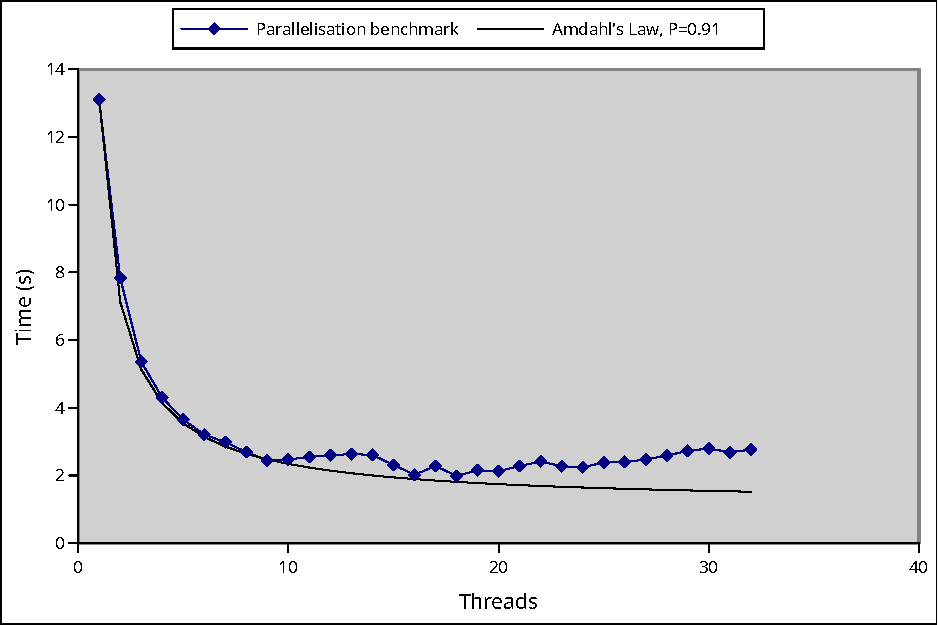
\includegraphics[width=\linewidth]{figures/parallel1.pdf}
   \caption{Time elapsed as a function of threads available and trendline according to Amdahl's Law (equation~\ref{eq:amdahl}).}
   \label{fig:parallel1}
   \end{subfigure}\quad\begin{subfigure}[b]{0.4\textwidth}
   \centering
   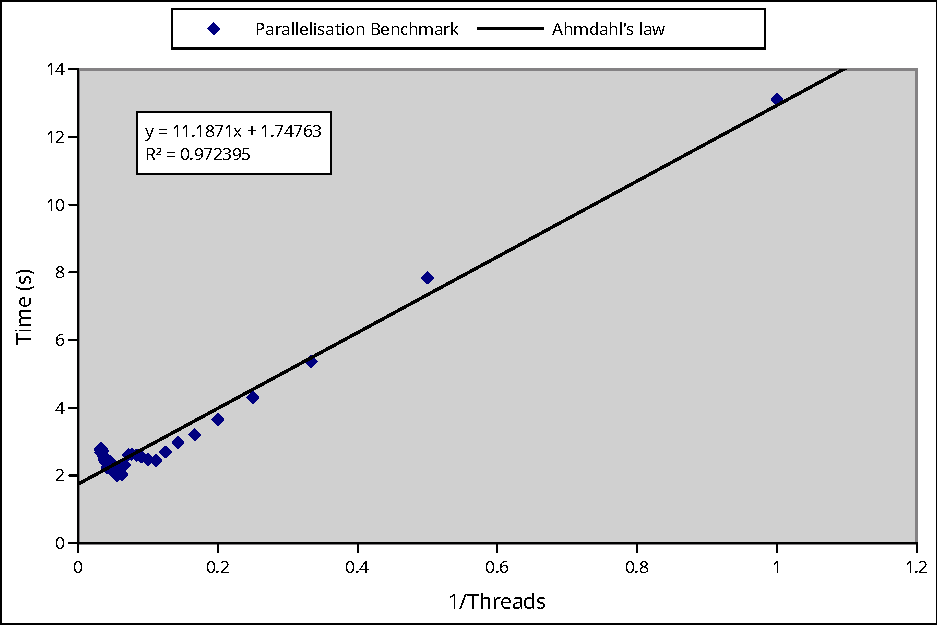
\includegraphics[width=\linewidth]{figures/parallel2.pdf}
       \caption{Time elapsed as a function of the reciprocal of threads available and linear lesat-squares regression.}
   \label{fig:parallel2}
   \end{subfigure}
   \caption{Parallelisation benchmark and Amdahl's Law.}
\end{figure*}

First the prallelisation is examined. The iPMCMC method is run on the model with $M=32$, $N=100$ and $R=10$, and the time elapsed is measured when running on a 32-core AMD Opteron 6274 machine. For each number of threads $1 \leq k \leq 32$, 10 measurements are taken and then averaged. The result is given in figure~\ref{fig:parallel1}. The data should follow Amdahl's Law~\cite{amdahl} for speedup as the number of cores available increases (or equivalently, the number of threads available assuming available cores). It is often formulated as the speedup acheived but might easily be reformulated into time elapsed \todo{Equation reference in figure}
\begin{equation}\label{eq:amdahl}
    T(k) = T(1)\left((1-P) + \frac 1 k P\right)
\end{equation}
for a given parallelisation $P$, which we want to find. The function is not linear in $k$, \todo{fixed $n$ instead of $k$} but is linear in $\frac 1 k$. This allows us to use linear least-squares regression to find $P$ if we plot the time elapsed agains the reciprocal of the number of threads available, see figure~\ref{fig:parallel2}. Both the slope $a$ and intercept $b$ may be used to calculate $P$, so the average of each method is used, giving approximately $P \approx 0.86$.

\subsection{Correctness}
\label{sub:correctness}

\begin{figure}[h]
    \centering
    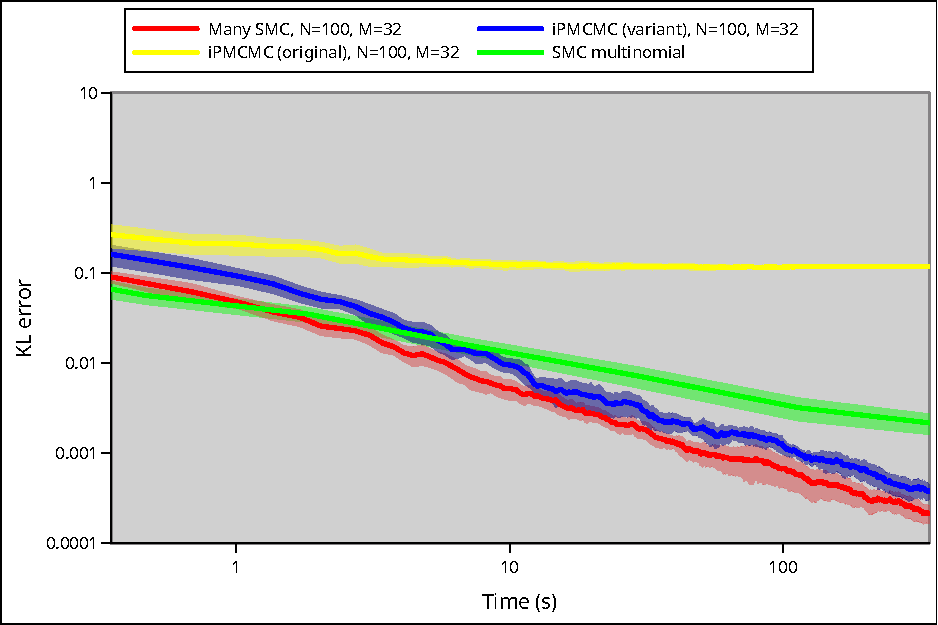
\includegraphics[width=\linewidth]{figures/correctness.pdf}
    \caption{Comparison of different methods: the \mbox{iPMCMC} sampler implemented in this thesis, a variant deviating from the specification, a trivially parallelisable sampler and a single SMC sampler.}
    \label{fig:corr}
\end{figure}

Correctness may be demonstated by comparing the results obtained from the method with the exact posterior distribution. For evaluation we choose $M=32$, $N=100$ and $R=1000$ where $M$ and $N$ are the same as the evaulation in the original article~\cite{ipmcmc} and $R$ is chosen to keep the testing time reasonable. \todo{Added number of threads used} For parallelisation, a value $k=20$ was chosen, motivated by the previous result. The sampler returns a list of samples for each iteration, allowing calculation of the error for any number of iterations $1 \leq r \leq R$ by taking the first $r$ elements of the result. For each $r$ the KL divergence is calulated according to equation~\ref{eq:kl}. To stabilize the results, the sampler is run 10 times and for each $r$ a 95\% confidence interval for the error is obtained. The result is given in figure~\ref{fig:corr}. For detailed runtime information, see appendix~\cite{sec:runtime}.

\todo[inline]{Added memory information. Perhaps a table?}.

The iPMCMC method implemented in this thesis is given by ``iPMCMC (original)''. It does not converge to the true posterior as it's not decreasing linearly but instead settles on some large error. It uses 33 MB of memory for a single run.

A variant ``iPMCMC (variant)'' that uses simple uniform sampling when selecting the nodes intestead of their marginal likelihood as decribed in section~\ref{sec:ipmcmc} shows the correct behaviour. It uses 659 MB of memory for a single run.

For reference, a single SMC sampler (the existing SMC sampler in Monad-Bayes) with increasing number of particles, ``SMC (multinomial)'' (12 MB for $N=4096$), and a trivially parallelisable alternative using no conditional samplers and uniformly sampling $P$ particles at each iteration (3121 MB), are also given.

\subsection{Evaluation}

The parallelisation described in section~\ref{ssub:parallelisation} is promising. The result indicated that over 80\% of the algorithm as implemented is parallelisable and the result in section~\ref{sub:correctness} shows that the variant algorithm outperforms the single SMC sampler after a few seconds.

The result of the original iPMCMC implementation is more troubling. The existence of bugs is evident by the incorrect behaviour expected on the log-log plot. The variant, only differing in how the next conditoinal nodes are sampled, shows where some of the bugs may be found. In addition, none of them are more performant than the trivially parallelisable alternative, possibly because of none of the iPMCMC methods correcty implements the algorithm described by Rainforth et al. The limitations described in section~\ref{sec:limits}, in particular only using a few of the generated particles, could also explain the difference.

\section{Conclusion}

This thesis shows that the approach by aggresively parallelising simpler samplers for use in MCMC methods is fruitful, evident by the performace comparison in figure~\ref{fig:corr} and the parallelisation analysis in section~\ref{ssub:parallelisation}. However the implementation of such methods are prone to error. The coordination of the many samplers is sensitive and great care have to be taken to not introduce bugs when implementing a procedure in functional code.

\subsection{Limitations}
\label{sec:limits}

The iPMCMC method implemented in this thesis is simplified. As written it only supports a subset of the models expressable in Monad-Bayes. To simplfy the resampling, only models containg the same number of scorings in every possible execution path are supported. In addition, the article by Rainforth et al. describes an approach for using all $MN$ generated trajectories each iteration instead of just $P$ trajectories. Finally the implementation could be made more performant. The pure nature of Haskell results much copying of data, but batched updates may be sped up in a safe way by performing mutation in the ST monad~\cite{stmonad}.

The evaluation only compares the implementation with samplers found in Monad-Bayes, in particular a comparison to other MCMC methods is missing. Another attractive comparison would be to the iPMCMC implementation in Anglican. Another aspect of the tests is the simplicity of the model. The models was chosen both because it has an exact calculatable posterior but also because it is fast. More complicated models, for example hidden Markov models, exists where the posterior is known.

\subsection{Future}

The points brought up on the previous section could be addressed in the future. More time could be spent on the implementation to eliminate the bugs and artifical limitations and truly evaluate the iPMCMC method in Monad-Bayes. 

The evaluation could be made more complete by comparing to additional methods and other probailistic programming languages. More models could also be tested to see if the trends apparent for the simple model carries over to more complex models.


%\bibliographystyle{author}

\printbibliography

\end{document}
